% !TEX TS-program = pdflatex
% !TEX encoding = UTF-8 Unicode

% This is a simple template for a LaTeX document using the "article" class.
% See "book", "report", "letter" for other types of document.

\documentclass[11pt]{article} % use larger type; default would be 10pt

\usepackage[utf8]{inputenc} % set input encoding (not needed with XeLaTeX)

%%% Examples of Article customizations
% These packages are optional, depending whether you want the features they provide.
% See the LaTeX Companion or other references for full information.

%%% PAGE DIMENSIONS
\usepackage{geometry} % to change the page dimensions
\geometry{a4paper} % or letterpaper (US) or a5paper or....
% \geometry{margin=2in} % for example, change the margins to 2 inches all round
% \geometry{landscape} % set up the page for landscape
%   read geometry.pdf for detailed page layout information

\usepackage{graphicx} % support the \includegraphics command and options

% \usepackage[parfill]{parskip} % Activate to begin paragraphs with an empty line rather than an indent

%%% PACKAGES
\usepackage{booktabs} % for much better looking tables
\usepackage{array} % for better arrays (eg matrices) in maths
%\usepackage{paralist} % very flexible & customisable lists (eg. enumerate/itemize, etc.)
\usepackage{verbatim} % adds environment for commenting out blocks of text & for better verbatim
\usepackage{subfig} % make it possible to include more than one captioned figure/table in a single float
% These packages are all incorporated in the memoir class to one degree or another...

%%% HEADERS & FOOTERS
\usepackage{fancyhdr} % This should be set AFTER setting up the page geometry
\pagestyle{fancy} % options: empty , plain , fancy
\renewcommand{\headrulewidth}{0pt} % customise the layout...
\lhead{}\chead{}\rhead{}
\lfoot{}\cfoot{\thepage}\rfoot{}

%%% SECTION TITLE APPEARANCE
\usepackage{sectsty}
\allsectionsfont{\sffamily\mdseries\upshape} % (See the fntguide.pdf for font help)
% (This matches ConTeXt defaults)

%%% ToC (table of contents) APPEARANCE
\usepackage[nottoc,notlof,notlot]{tocbibind} % Put the bibliography in the ToC
\usepackage[titles,subfigure]{tocloft} % Alter the style of the Table of Contents
\renewcommand{\cftsecfont}{\rmfamily\mdseries\upshape}
\renewcommand{\cftsecpagefont}{\rmfamily\mdseries\upshape} % No bold!

%%% END Article customizations

\usepackage[spanish]{babel}
\usepackage{listings} 
%%% The "real" document content comes below...

\title{Investigación de Lenguajes - Python}

%\date{} % Activate to display a given date or no date (if empty),
         % otherwise the current date is printed 

\begin{document}
\maketitle
%\tableofcontents % No hace falta un TOC en un artículo corto
\begin{itemize}
\item Leonel Ramirez
\item José Vélez
\item Kevin Campuzano
\end{itemize}

\section{Introducción}
Python es un lenguaje de programación diseñada por el europeo Guido Van Rossum en el año 1991, tomando ideas prestadas de los lenguajes de programación que conocía por ejemplo ABC y lenguaje de programación Haskell.
Destaca sus características que le han llevado a ser un lenguaje muy conocido hoy en día, también por ser de código abierto administrado por Python Software Foundation, El nombre de Python fue inspirado por la serie The Monty Python de la BBC de Londres.
Es un lenguaje scripting independiente de plataforma y orientado a objetos  por lo tanto está preparado para soportar cualquier tipo de programa, como aplicaciones Windows a servidores de red hasta páginas web.
Python es mantenido por un numeroso grupo de voluntarios en todo el mundo por ser un software de código abierto.  También es un lenguaje interpretado quiere decir que no necesita compilar el código fuente para poder ejecutar, una de las ventajas que ofrece es su rapidez de desarrollo.
\begin{figure}[htbp]
\begin{center}
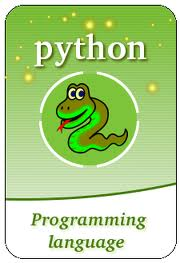
\includegraphics[width=.30\textwidth]{./imagenes/pythonXD.jpg}
\caption{python}
\label{qt}
\end{center}
\end{figure}

\section{Características}

\textbf{Sencillo de Aprender}
\\    Python es extremadamente sencillo de iniciarse en la programación ya que ofrece una sintaxis extraordinariamente simple.\\

\textbf{Lenguaje de Alto Nivel}
\\    Cuando escribes programas en Python nunca debes preocuparte por detalles de bajo nivel, como manejar la memoria empleada por tu programa.\\

\textbf{Sintaxis de Python}
\\	  Es muy elegante y permite la escritura de programas cuya lectura resulta sencilla.\\

\textbf{Librerías Extendidas}
\\	  La librería estándar de Python es de hecho muy amplia. Puede ayudarte a hacer varias cosas que involucran: expresiones regulares, generación de documentos, evaluación de unidades, pruebas, procesos, bases de datos, navegadores web, CGI, ftp, correo electrónico, XML, XML-RPC, HTML, archivos WAV, criptografía, GUI(graphical user interfaces/interfase grafica del usuario) usando Tk, y también otras funciones dependientes del Sistema.\\

\textbf{Incrustable}
\\    Puedes insertar Python dentro de tu programa en C/C++ para ofrecer las facilidades de "scripting" dentro del mismo.\\

\textbf{Tipado Dinámico}
\\    No es necesario declarar tipo de dato que contiene una variables , este se asigna automáticamente al darle un valor a la variable.\\

\textbf{Multiplaforma}
\\   Disponible para sistemas operativos Unix, GNU/Linux, Solaris, Mac OS, Windows, entre otros.\\

\textbf{Fuertemente Tipado}
\\   No se permite tratar a una variable como si fuera de un tipo diferente.\\

\textbf{Multiparadigma}
\\   Python es un lenguaje orientado a objetos pero también permite usar otros paradigmas de programación tales como programación estructurada, programación funcional y programación orientada a aspectos.\\

\section{Historia}
\begin{figure}[htbp]
	\begin{center}
		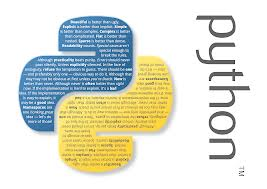
\includegraphics[width=.60\textwidth]{./imagenes/python.png}
		\caption{Logo}
		\label{Logo}
	\end{center}
\end{figure}

Python fue lanzado por primera vez en 1991, desarrolado por Guido van Rossum, un programador de origen holandés que desarrolló este lenguaje de programación a finales de los años 80 para el Centro para las Matemáticas y la Informática de los Países Bajos que buscaba un lenguaje de programación para ser utilizado bajo el sistema operativo Amoeba de Andrew S. Tanenbaum que fuese capaz de sustituir al lenguaje ABC.
\\\\
Python es un proyecto de codigo abierto, administrado por la Python Software Foundation.
\\\\
Python es un lenguaje de programación de alto nivel que fue diseñado con una sintaxis muy limpia que permitiese obtener códigos que fuesen fáciles de leer, es multiplataforma y soporta orientación a objetos, programación imperativa e, incluso, programación funcional.
\\\\
Se puede utilizar para muchos tipos de desarollo de software. El proposito del diseño del lenguaje Pyhton hace hincapie en  la productividad del programador y legibilidad del codigo.
\\\\
Su nombre fue inspirado el la seria THE MONTY PYTHON de la BBC de Londres.
\\\\
Hoy en dia, Python es mantenido por un numeroso grupo de voluntarios en todo el mundo.


\begin{figure}[htbp]
	\begin{center}
		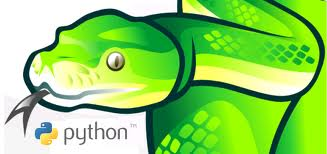
\includegraphics[width=.50\textwidth]{./imagenes/python1.png}
		\caption{python}
		\label{python}
	\end{center}
\end{figure}

\section{Tutorial de Instalación}

Tutorial como Instalar Python en Windows\\
 

1.	Identifica la versión de Windows que se ejecuta en tu PC. Tienes que saber  si maquina está ejecutando Windows 95, 98, NT, 2000, ME, XP, Vista o Windows 7.\\

2.	Decide si necesitarás el código fuente de Python bueno se recomienda que la instale. Instalar la fuente es opcional. Python es un software de código abierto, lo que significa que el código está disponible para los programadores para modificar o distribuir a su antojo.\\

3.	Entrar a la página web Python.org. Todas las distribuciones oficiales del programa se pueden encontrar aquí, incluyendo un archivo. Msi instalador para Windows.\\

4.	Haz clic en el enlace "Descargar". Una lista de archivos aparecerá. Cada archivo es una distribución de Python para una plataforma específica.\\

5.	Encuentra el .exe o instalador para la versión de Windows que tienes instalada en un tu máquina.  Numerosas versiones de Python están disponibles para entornos Windows.\\


6.	En las versiones actuales de Windows todos las archivos que bajes de la red se alojaran en una carpeta llamada descarga la puedes encontrar en tus archivos, es ahí donde se guardara el instalador de Python.\\  

Ejecuta el instalador\\

1.	Ejecuta el instalador. Busca el archivo. Msi usando Windows explorer y ejecútalo. Un programa de instalación se abrirá. Haz clic en Instalar para todos los usuarios y luego en Siguiente.\\

2.	Escoge un directorio de instalación para Python. El valor por defecto, "C: \ Python25", se recomienda dejar el mismo directorio si tienen experiencias instalando programas.\\

3.	Elige las funciones que deseas instalar y haz clic en "Siguiente" para iniciar la instalación. Espera un momento hasta que se complete la instalación. Una vez que se haya instalado Python, haz clic en "Finalizar".\\

4.	Haz clic en Programas, Python 2.5 luego Python desde el menú Inicio de Windows para probarlo. Una ventana en negro y blanco se abrirá con un comando interactivo de Python del sistema. Una vez que hayas confirmado que el programa está instalado correctamente, cierra la ventana.\\

5.	Haciendo clic en Inicio y luego en Ejecutar. Cuando el diálogo se abra, escribe cmd en el cuadro de búsqueda y presiona Aceptar. Ejecutar los programas de Python desde la línea de comandos es una forma útil de ver el destino y pasar parámetros aunque se necesita un poco de practica para dominar la ventana de comandos.\\

6.	Cambia a tu directorio de Python. Si aceptas el directorio por defecto, escribe cd,  C: \ Python25" en el prompt del comando y presiona Enter. Si lo has instalado en otro lugar, cambia C: \ Python25 a la carpeta de instalación. Escribe python y presiona Enter para iniciar la línea de comandos de Python del sistema.\\


\section{Hola Mundo y otros Programas Introductorios}

 Programa Factorial
  \\  
 Se resolvera en forma recursiva


\lstset{language=Pascal}          % Set your language (you can change the language for each code-block optionally)

\begin{lstlisting}[frame=single]  % Start your code-block
for i:=maxint to 0 do

def fibonacci(contador,n,p1,p2):
  var = ""
   if(contador!=n):
   	var=fibonacci(contador+1,n,p2,p1+p2)
   	var=str(p2)+" "+var
   return var
n= int(input("Ingrese un numero entero\n"))
if(n>0):
 a=fibonacci(0,(n-1),0,1)
 print("0 "+a)  
\end{lstlisting}


\newpage
 Programa Fibonacci

\begin{lstlisting}[frame=single]  % Start your code-block
for i:=maxint to 0 do
def factorial(x,n):
  if(n>0):
   x=factorial(x,n-1)
   x=x*n
  else
   x=1
  return x
 n= int(input("ingresa un numero  \n"))
 x=1
 x=factorial(x,n)
 print(x)
\end{lstlisting}



\end{document}
